\documentclass[a4paper, 12pt]{article}

% Packages
\usepackage[utf8]{inputenc} % UTF-8 encoding
\usepackage[T1]{fontenc}    % Font encoding
\usepackage[english]{babel}  % Language
\usepackage{graphicx}       % For including images
\usepackage{amsmath}        % Math packages
\usepackage{amsfonts}
\usepackage{amssymb}
\usepackage{natbib}         % Bibliography package
\usepackage{url}            % URL formatting
\usepackage{hyperref}       % Hyperlinks
\usepackage{geometry}       % Adjust page margins
\usepackage{setspace}       % Adjust line spacing

\graphicspath{{Images/}}

% Title and Author
\title{Survey of Strontium Isotope Analysis in Archaeological Research of Ancient Egypt}
\author{Jaxon Lee}
\date{\today}

\begin{document}

\maketitle

\begin{abstract}
    This paper explores the pivotal role of strontium isotope analysis in
    reshaping our understanding of ancient Egyptian history. It delves into
    the methodology, purpose, and applications of this analytical approach,
    emphasizing its ability to discern geographic origins and trace human movements.
\end{abstract}

\section{Introduction}
The exploration of ancient Egyptian civilization has been significantly enhanced by
advancements in analytical techniques, particularly the application of strontium
isotope analysis. This paper navigates the transformative role of strontium isotope
studies in augmenting our comprehension of ancient Egyptian history.

Archaeologists routinely unearth human skeletal remains, and one valuable tool for
elucidating more about them is isotope analysis. This involves investigating the
levels of various elements such as oxygen, carbon, or strontium using chemistry.
Strontium isotope analysis, in particular, proves indispensable for archaeologists
as it facilitates an understanding of the geographic movement of humans and animals.

Over the last decade, strontium isotope analysis has gained substantial momentum,
propelled by advancements in measuring technology \citep{holt2021}. Since a
comprehensive study of strontium isotope analysis and its broad application to archaeology
exceeds the scope of this paper, my focus centers on its relevance to archaeological
research in ancient Egypt. This choice is driven by the intriguing application of
strontium isotope analysis to Egyptian mummies.

Within the confines of ancient Egypt, a rich array of questions has emerged, leading
to insightful revelations through strontium isotope analysis. This paper aims to
illuminate how strontium isotope analysis functions, its primary use cases, and several
compelling case studies that leverage its potential.

\section{Strontium Isotope Analysis}
\subsection{Overview}
\begin{figure}[htbp]
    \centering
    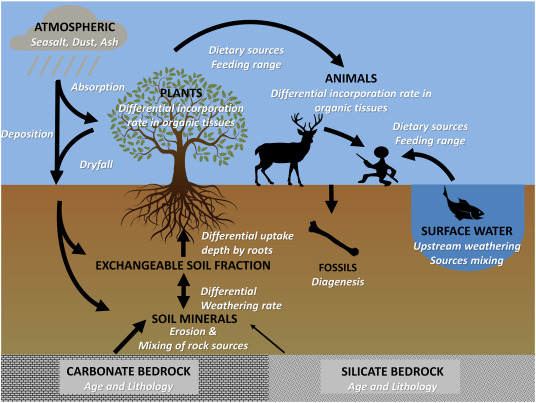
\includegraphics[width=0.8\textwidth]{strontium_process.jpg}
    \caption{A depiction of how strontium goes from bedrock into the ecosystem, where every arrow
        represents the movement of strontium \citep{bataille2020}}
    \label{fig:strontium_process}
\end{figure}

Strontium is an element, which occurs naturally at varying concentrations in rock formations.
Strontium gets into the water stream through erosion and eventually is inadvertently consumed by plants and animals in trace amounts \citep{bartelink2019}.
Eventually, when humans or animals inevitably consume plants, water, or other animals,
a small amount of strontium gets into their bones and tissue. Notably, although the amount is trace, the
ratio of strontium isotopes remains constant throughout these processes since there is no "isotopic fractionation" \citep{bartelink2019}.
Thus, measuring strontium in bones or tissue gives a picture of where humans or animals source their food and water.
The process by which strontium goes through an ecosystem is shown in Figure~\ref{fig:strontium_process}.

\subsection{How It Works}

Now, I will detail the underlying principles behind strontium isotope analysis
and how to perform it.
First, an "isotope" is a version of an element with a particular atomic weight,
which is indicated by a superscripted number to the left of the elemental symbol \citep{Meave60_2015}.
For example, one isotope of Oxygen is \textsuperscript{18}O, where 18 represents
the atomic weight of the isotope. There are four possible isotopes of strontium in
nature \citep{holt2021}, but only two are relevant to strontium isotope analysis: \textsuperscript{87}Sr and \textsuperscript{86}Sr.
Notably, these isotopes are extremely stable. They do not react with other elements,
and their abundance in the environment will stay constant unless outside forces interfere \citep{Long1998}.

One such outside force is the radioactivity of \textsuperscript{87}Rb, which forms \textsuperscript{87}Sr when it decays. So, the \textsuperscript{87}Sr concentration in a substance
will increase over time depending on the initial concentration of \textsuperscript{87}Rb.
\textsuperscript{87}Rb has a half-life of 48.8 billion years \citep{holt2021}, so it takes billions of years
for \textsuperscript{87}Rb to fully decay into \textsuperscript{87}Sr; as a result, \textsuperscript{87}Rb will always
have a small but measurable effect on the \textsuperscript{87}Sr levels of its containing
substance.
Thus, the ratio of \textsuperscript{87}Sr / \textsuperscript{86}Sr
increases variably depending on \textsuperscript{87}Rb concentrations.

And, \textsuperscript{87}Rb varies significantly across the environment.
This is because of how rocks form; in deep Earth layers, magma mixes and moves constantly,
which spreads and changes \textsuperscript{87}Rb concentrations.
In addition, when the magma cools,
\textsuperscript{87}Rb will spread out irregularly due to its chemical properties \citep{holt2021}.
Therefore, different rock formations will have more
\textsuperscript{87}Sr than \textsuperscript{86}Sr depending on a complex mix of
the movement and mixing of the magma that formed it, the irregular permeating of
\textsuperscript{87}Rb during formation, and the initial concentrations of \textsuperscript{87}Sr and \textsuperscript{86}Sr \citep{Long1998}.
Researchers can quantify the relative levels of \textsuperscript{87}Sr and
\textsuperscript{86}Sr by measuring their ratio.


For archaeological purposes, we can assume that every rock has a random, unique
ratio of \textsuperscript{87}Sr to \textsuperscript{86}Sr. As stated previously,
both isotopes eventually travel through the ecosystem to all nearby
plants and animals. Researchers have found that strontium isotope ratios do not
"fractionate," or meaningfully change, at any point in its journey through
the ecosystem \cite{bartelink2019}. As a result, the strontium isotope ratios that are
incorporated into human, animal, and plant tissue reflect the strontium isotope
ratios of the preceding trophic level almost exactly. Assuming a closed ecosystem
with a single environmental strontium ratio,
the strontium isotope ratios of the entire ecosystem would be homogenous.

To measure the ratio of \textsuperscript{87}Sr / \textsuperscript{86}Sr, archaeologists must first
destructively procure a sample. Archaeologists usually select molar teeth
for sampling in humans and animals. Then, the sample must be cleaned both physically and chemically to avoid
contamination. Finally, archaeologists dissolve the sample in acid and
use a mass spectrometer to determine the
\textsuperscript{87}Sr / \textsuperscript{86}Sr ratio \citep{Long1998}

In summary, \textsuperscript{87}Sr / \textsuperscript{86}Sr ratios can serve as a
"fingerprint" for identifying geographic areas since they vary greatly
across the environment. This is useful for archaeologists because strontium isotope ratios
can be measured in organic material to get an idea of where the tissue was when it formed.
Also, strontium isotopes are stable once formed. Thus, measuring strontium isotope ratios is
desirable because sources of error are limited.


\subsection{Purpose}
The main use of strontium isotope analysis in Egyptian archaeology is to understand
"provenance," or place of origin. Since most bones remold over time, measuring their
strontium levels gives insight into the last 7-10
years of a person's life. Measuring the strontium ratios of human hair can elucidate a person's
geographical residence immediately before death \citep{kamenov2014}. Although this is trivially useful for fields such as forensics \citep{kamenov2014},
archaeologists know where people were when they died
since people are usually buried where they lived. However, since tooth enamel
forms during childhood and does not change, measuring it can give the general location
that the person lived in during their tooth formation, i.e., when they were a child
\citep*{holt2021,kozieradzkaogunmakin2021,lazzerini2021}. Thus, archaeologists can
identify the provenance of skeletal remains they dig up so long as they have access
to tooth enamel samples.

\subsection{Isoscapes}
% How they make isoscapes
For strontium isotope measurements of organic tissue to be useful, archaeologists need to know
which ratios correspond to which places.
So, archaeologists create "isoscapes," which are maps of the expected
\textsuperscript{87}Sr / \textsuperscript{86}Sr ratios
of samples in various geographic regions. This creates a baseline that other archaeologists
can compare against when doing strontium analyses. I will discuss the three main approaches
for creating isoscapes: domain mapping,
contour mapping, and machine learning \citep{holt2021}. I will also go over their
strengths and weaknesses.
\subsubsection{Domain Mapping}
\begin{figure}[htbp]
    \centering
    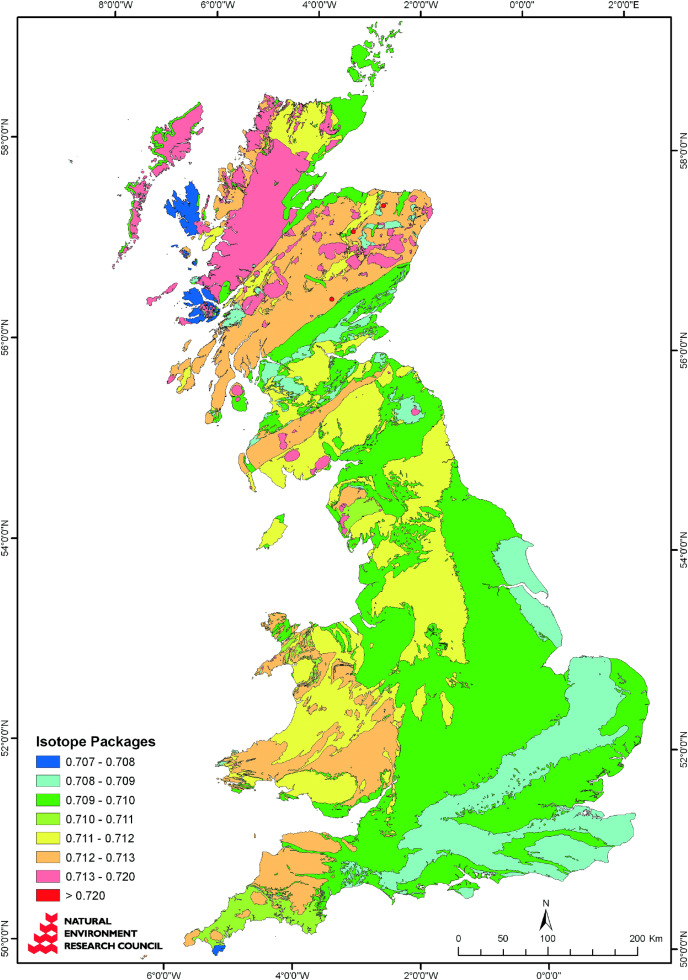
\includegraphics[width=0.45\textwidth]{domain_mapping.jpg}
    \caption{A domain map of Great Britain \citep{evans2010}}
    \label{fig:domain_mapping}
\end{figure}
To make a domain map, researchers sample the strontium isotope ratios of
various locations, plot the results on a map, and then group similar results
together by hand into "domains." Usually, researchers take multiple samples
in each region and average them to ensure outliers do not throw off the results.
This is the simplest approach to creating an isoscape, but it is expensive due to the number
of samples needed to cover a geographic area. For this reason,
domains usually have low resolution—in other words, broad ranges—due to
limited time and money to sample regions.
Despite this, domain mapping is generally considered the best isoscape approach \citep{holt2021}.
An example of a domain map can be seen in Figure~\ref{fig:domain_mapping}.


\begin{center}
    \begin{tabular}{||c | c||}
        \hline
        Advantages            & Disadvantages            \\ [0.5ex]
        \hline\hline
        Easy to make          & Imprecise                \\
        \hline
        Simple to interpret   & Requires lots of samples \\
        \hline
        Fast to use once made & Expensive                \\
        \hline
                              & Time consuming           \\ [1ex]
        \hline
    \end{tabular}
\end{center}

\subsubsection{Contour Mapping}
\begin{figure}[htbp]
    \centering
    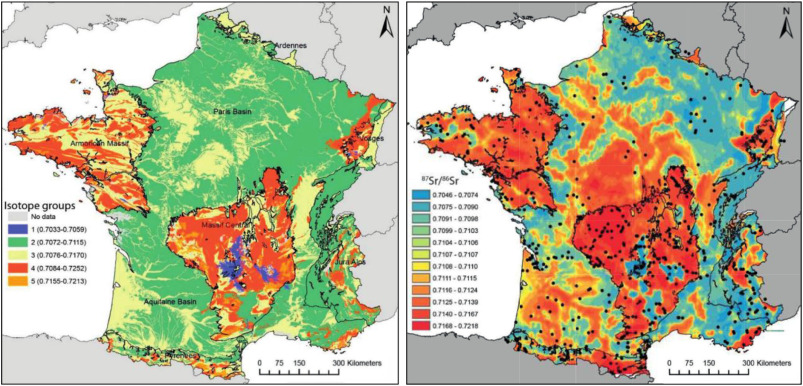
\includegraphics[width=0.9\textwidth]{contour_mapping.jpg}
    \caption{A domain map of France (left) versus a contour map of France (right) \citep{willmes2018}}
    \label{fig:contour_mapping}
\end{figure}

For contour maps, researchers take \textsuperscript{87}Sr / \textsuperscript{86}Sr
samples just as they would for domain mapping, but they use statistics to extrapolate
strontium isotope ratios between the sampling areas instead of grouping similar results
by hand. This can greatly increase resolution and reduce the number of samples needed to make a full isoscape. Some statistical
methods that researchers use for contour mapping are inverse distance weighting, ordinary kriging, empirical Bayesian kriging,
and cokriging \citep{holt2021}. Unfortunately, researchers agree that this approach is ineffective
because strontium ratios do not gradually change between sampling areas. In reality,
they have sharp drop-offs due to the underlying rock formations \citep{holt2021}, which
no statistical method can predict. A contour map is shown along with a domain map of the same
area in Figure~\ref{fig:contour_mapping}. As can be seen, the contour map has more
fluid boundaries and twice as much resolution when compared with the domain map.

\begin{center}
    \begin{tabular}{||c | c||}
        \hline
        Advantages             & Disadvantages                       \\ [0.5ex]
        \hline\hline
        High resolution        & Generally inaccurate                \\
        \hline
        Can give exact results & Can generate impossible results     \\
        \hline
        Relatively cheap       & Unreliable                          \\
        \hline
                               & Can not predict sharp ratio cutoffs \\[1ex]
        \hline
    \end{tabular}
\end{center}

\subsubsection{Machine Learning}
\begin{figure}[htbp]
    \centering
    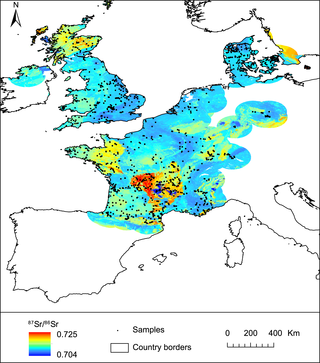
\includegraphics[width=0.5\textwidth]{machine_learning_isoscape.png}
    \caption{A machine-learning-based isoscape of Western Europe \citep{bataille2018}}
    \label{fig:machine_learning}
\end{figure}
For machine learning-based approaches, researchers use algorithms
that learn how to predict
strontium isotope ratios based on existing strontium samples, models of natural processes such as chemical weathering, and
environmental data like geological maps \citep{bataille2018}. The key difference between
this approach and contour mapping is the ability to factor in more types of data.
One example of a machine learning algorithm used for this purpose is random forest regression
\citep{bataille2018}. Notably, machine learning algorithms are capable of predicting
the sharp drop-offs we expect from strontium ratios in isoscapes, which contrasts
with contour mapping approaches. Furthermore, machine-learning-based approaches are
capable of displaying the confidence of a particular measurement or region of
measurements; this allows researchers to gauge how much they should trust a measurement
and also give ideas on where to sample next to improve the isoscape.
Early results show that these models can be extremely effective at producing accurate
isoscapes. However, these algorithms are complex, are still being proven, and have
yet to be applied globally. An example of an isoscape generated by random forest
regression can be seen in Figure~\ref{fig:machine_learning}.

\begin{center}
    \begin{tabular}{||c | c||}
        \hline
        Advantages                              & Disadvantages                  \\ [0.5ex]
        \hline\hline
        High resolution                         & Complicated to make            \\
        \hline
        Can predict sharp ratio cutoffs         & Computationally intensive      \\
        \hline
        Extremely accurate                      & Not fully fleshed out          \\
        \hline
        Gives prediction confidence             & Needs lots of extra data       \\
        \hline
        Additional variables can be factored in & Limited applications presently \\[1ex]
        \hline
    \end{tabular}
\end{center}


\subsection{History}
I will briefly explain the origins of strontium isotope analysis, major advancements,
and where the method is trending. Originally, strontium isotope analysis was used to age rocks, study erosion, and
find the source of rivers \citep*{moorbath1965, crowley2017}. Around the late 1980s and early 1990s, archaeologists theorized
that they could use strontium isotope analysis of tooth enamel to find human provenance \citep{crowley2017}. This spawned
a flood of studies to prove its viability and test its limitations \citep{crowley2017}.
Since then, archaeologists have increasingly used strontium isotope analysis to answer
questions of human origins. Recently, there has been an explosion of strontium
isotope analysis research \citep{crowley2017}; scientific
breakthroughs such as high performance laser ablation and multicollector inductively coupled
plasma mass spectrometry and increasing availability of high-quality isoscapes \citep{crowley2017}
have made strontium isotope analysis more accessible and more effective \citep{holt2021}.
According to \cite{holt2021}, the main focus of strontium research now is creating new isoscapes
and refining existing ones. The advent of machine learning-based approaches to isoscapes
is particularly interesting as it could drastically increase the resolution of isoscape
baselines and potentially allow for more specific regional identification from strontium
isotope analysis.


\subsection{Limitations}
The main weaknesses of strontium isotope analysis are accuracy, precision, and cost.
\subsubsection{Accuracy}
Strontium isotope analysis can be inaccurate. A person consistently moving
across geological areas during childhood will make their tooth enamel strontium ratios
indiscernible.
But, this amount of mobility was uncommon in history and often infeasible, so archaeologists
generally ignore this possibility.
Also, people might source their food and water from a different geographic region from where
they lived, which could throw off results.
This is further complicated by plant consumption disproportionately affecting strontium ratios \citep{price2006}.
So, even if the majority of a
person's diet consisted of local food and water, a relatively
small amount of non-local farm products could give a false negative on a locality test.
But, if one understands what historical people ate and where they got their food,
one can account for these dietary effects in one's strontium isotope analysis.



\subsubsection{Precision}
Strontium isotope analysis can give results that are too broad. In many parts of the world, isoscapes are not
refined or have low resolution \citep{holt2021}.
So, strontium measurements only give a general region of provenance, which is sometimes insufficient to answer a research question.
However, this can be alleviated by combining strontium isotope analysis with other tools,
such as analyzing isotopes of \textsuperscript{13}C, \textsuperscript{18}O, and \textsuperscript{34}S
to understand diet, climate, and likely distance to a water source respectively \citep{madgwick2019}.
If multiple sources of data corroborate the same conclusion,
the conclusion is likely to be valid.

\subsubsection{Price}
Strontium isotope analysis is expensive \citep{holt2021}. It involves highly specialized tools along
with expertise in chemistry to operate them. Furthermore, researchers must take many samples to get
meaningful results. The best approach to mitigate this
is to apply strontium isotope analysis only where needed and leverage its results
as much as possible. Nevertheless, advancements in technology will
enhance the cost-effectiveness and efficacy of strontium isotope analysis,
which instills optimism for its future prospects.


\section{Use Cases}
In this section, I will discuss the main questions supported by strontium isotope
analysis in the context of ancient Egyptian archaeology. I will follow this
by describing the method's use cases beyond archaeology since this may give
archaeologists ideas for future applications.

\subsection{Archaeological Use Cases}
\subsubsection{Local vs Non-Local Humans}
Since strontium isotope analysis can give low-resolution results, Egyptian archaeologists
often simplify their provenance question to "local," or from the area under study,
and "non-local." For example, archaeologists can measure the
\textsuperscript{87}Sr / \textsuperscript{86}Sr ratio
of human remains in a graveyard and then track the proportion of local and
non-local people \citep{holt2021}. This approach does not require
a perfect isoscape since researchers do not need to know exactly where non-local
individuals came from so long as the strontium ratios of the local area are understood and the non-local
strontium ratios are sufficiently different from local ones. This increases the accuracy of results, but it limits the breadth
of questions that can be answered with strontium isotope analysis.


\subsubsection{Migration and Movement}
Provenance studies can give insight into the mobility of ancient cultures. Researchers
can identify the distance and frequency of travel among a group of subjects. As an example, \cite{copeland2011} found that early human females were more likely
to be non-local than early human males based on a strontium isotope analysis.
This indicates gendered mobility in prehistory; early females were more likely to travel whereas early males
were more likely to be sedentary.

\subsubsection{Historical Animal Origins}
Archaeologists also study animal remains
to find their origins. This can reveal societal trading patterns. For example, in the work of \cite{arnold2016}, researchers investigated strontium isotope ratios of
farm animals in Israel, and they found clear evidence of
Egyptian strontium ratios in the animals' tooth enamel. Since the animals predate
the previously known animal trade by hundreds of years, the researchers concluded
that early Israelis and Egyptians traded these animals long before previously understood.

\subsubsection{Agricultural Products}
Archaeologists can study strontium isotope ratios in crops to determine their origins.
For instance, \cite{larsson2020} studied the
origins of historic farm produce of Uppåkra in Sweden with strontium isotope analysis.
They found non-local crops, which
gave insight into the trade and movement of the culture under study.
Of course, similar analyses could be conducted for ancient Egypt.


\subsubsection{Material Origins}
More rarely, Egyptian archaeologists use strontium isotope analysis to determine the origin
of physical artifacts. For example, \cite{barfod2020} concluded that celebrated
clear glass in Roman cities came from Egypt.



\subsection{Other Use Cases}
\subsubsection{Forensics}
Strontium isotope analysis can be used to learn more about the body of a
deceased victim. Scientists can uncover information about the place of origin
of a body, which could help identify it even if it is unrecognizable. For example,
\cite{kamenov2014} used strontium isotope analysis along with other isotopic
analyses on a decades-old cold murder case of an unidentified woman in Florida.
Although the researchers could not conclude the identity of the victim, they
found she likely originated in Europe and arrived in Florida less than a year
before she died. This gave investigators new leads, and the case was
reopened and actively under investigation at the time of the research article.


\subsubsection{Illegally Poached Animals}
Researchers can gain insights into the origins of poached animal products after
they get to market. This helps authorities find and shut down illegal poaching
operations, which has ramifications for conservation. For instance, \cite{singh2006}
presents an approach for determining if ivory was sourced from Asian elephants or African elephants based
on strontium isotope analysis in addition to other metrics.
Unfortunately, researchers rarely use
strontium isotope analysis for these ends. This is likely because the result resolution is low,
and authorities usually already know the general area of provenance for poached animals.
However, I expect strontium isotope analysis to increase its relevance in this
area as methods improve.


\subsubsection{Range of Invasive Species}
To understand the spread and impact of invasive species in different regions,
researchers can use strontium isotope analysis to find where an invasive
specimen originated in the hopes of tracking their movement. \cite{wolff2012} apply this principle
to track invasive fish in the Upper Colorado River Basin, which aided the population
control efforts of authorities.

\section{Case Studies}
Now, I will go over three interesting case studies on ancient Egyptian archaeology
that utilize strontium isotope analysis. Ideally, this will give archaeologists ideas on how to apply strontium isotope analysis to
their work.
\subsection{The Hyksos' Rise to Power}
% Hyksos

\begin{figure}[htbp]
    \centering
    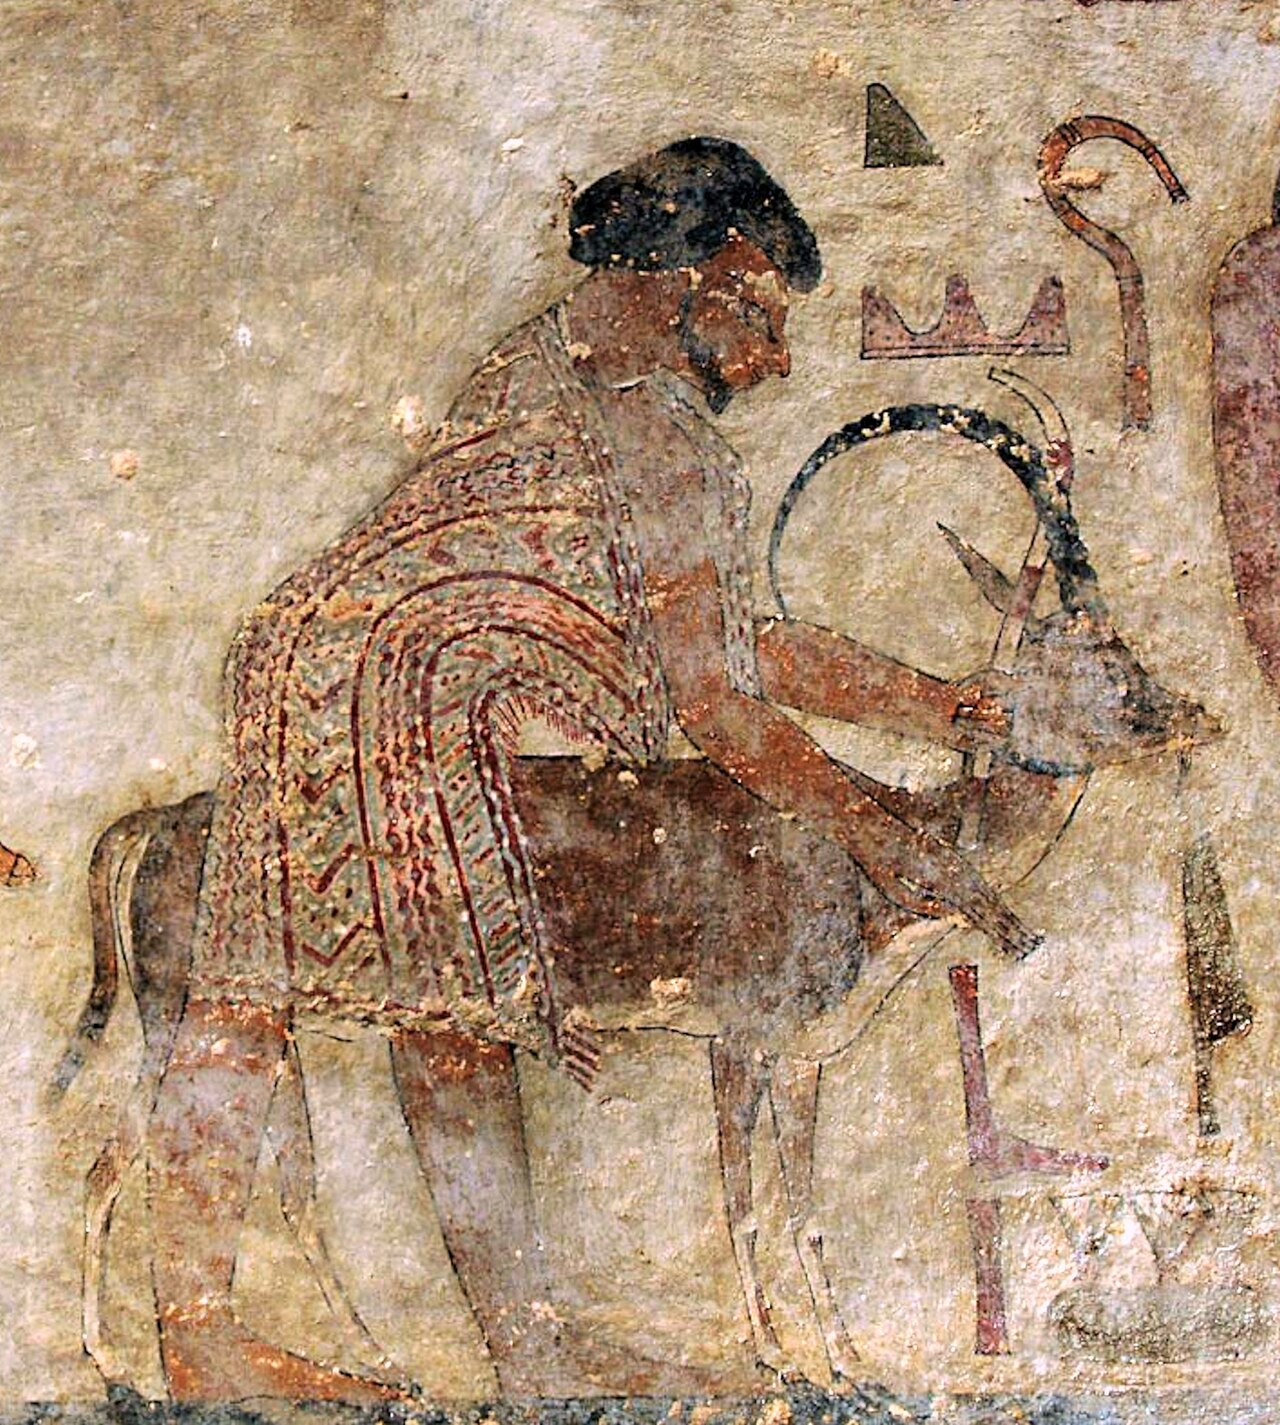
\includegraphics[width=0.5\textwidth]{hyksos_painting.jpg}
    \caption{Egyptian painting of Abisha the Hyksos \citep{wikipediaHyksos}}
    \label{fig:hyksos_painting}
\end{figure}
During the period of 1638 BCE to 1530 BCE, the foreign Hyksos people rose to power
and ruled over Egypt. What little we know about this comes
from a single ancient Egyptian priest named Manetho hundreds of years after the Hyksos were gone. He
claimed that the Hyksos were oppressive rulers who seized power through invasion \citep{stantis2020}.
An ancient picture of a Hyksos ruler is in Figure~\ref{fig:hyksos_painting}. There are a wealth
of resources on applying strontium isotope analysis to the origins of the Hyksos \citep*{stantis2020, stantis2021, weinstein2021, maaranen2019}.
I have selected the one I found the most interesting. In a research article from 2020, \cite{stantis2020} challenge
Manetho's narrative
using evidence from strontium isotope analysis.

The researchers first sought after the graves of people who lived during and immediately
before the Hyksos period. They decided to excavate a cemetery in Tell el-Dab'a,
which was the capital of the Hyksos kingdom. The cemetery had generations of Egyptians
with burials spanning 500 years before and during the Hyksos rule.

Then, the researchers sampled tooth enamel from these skeletons to see if they fell
in the "local" range of strontium ratios. Specifically, they analyzed second permanent molars,
first permanent premolars, and second permanent premolars. 75 skeletons were analyzed;
half were buried before Hyksos rule and half were buried during Hyksos rule.

The researchers found that there were numerous non-local people from a wide range
of places across all time periods. About half of all skeletons studied were non-local
according to their strontium isotope ratios, and most of the non-local people were buried
before Hyksos rule. Further, women were disproportionately non-local.

Thus, the researchers concluded that the Hyksos did not invade Egypt
as the ancient priest Manetho asserted. The researchers argue that the Hyksos
arrived centuries before and gradually rose to power. This is supported
by increasing amounts of non-local people before the Hyksos ruling
period. If the Hyksos seized power through invasion, one would expect few non-local
people before Hyksos rule and a large amount of non-local people immediately after they conquered Egypt, which
is not the case. The disproportionate number of non-local women also supports this conclusion
as an invading force would consist of non-local men.

The work of \cite{stantis2020} shows the main strength of strontium isotope analysis:
identifying provenance. They also reveal the method's versatility; researchers can
apply provenance to answer other, more nuanced questions such as the causes of
power dynamics in ancient societies. Finally, the article explains how strontium isotope
analysis can provide rare scientific evidence to support or contradict
historical accounts, which is usually challenging to achieve.


\subsection{Mummified Birds}
% Mummified Birds
\begin{figure}[htbp]
    \centering
    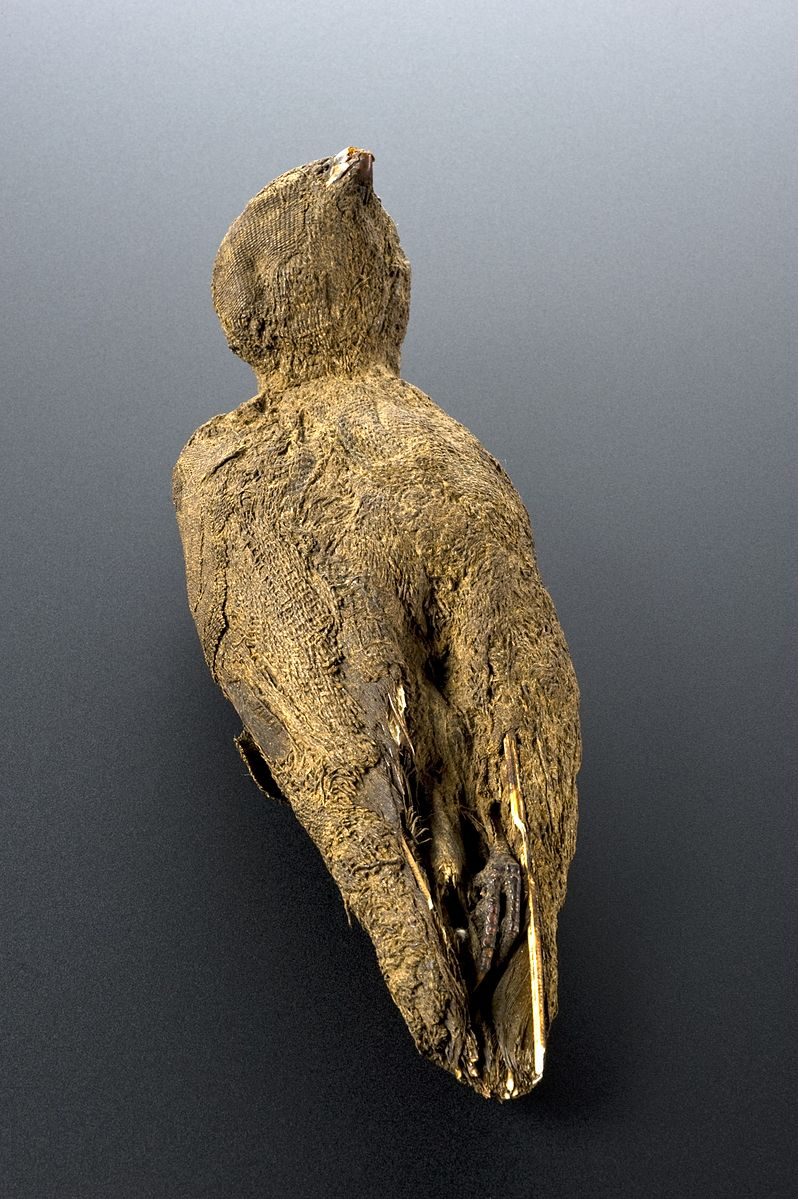
\includegraphics[width=0.35\textwidth]{mummy_bird.jpg}
    \caption{An ancient Egyptian mummified bird \citep{wikipediaBird}}
    \label{fig:mummy_bird}
\end{figure}
In addition to human mummies, ancient Egyptians sometimes mummified birds
like ibises or birds of prey. This honored gods who took
the forms of birds, such as Horus and Thoth. One example of a mummified bird is in Figure~\ref{fig:mummy_bird}.
\cite{linglin2020} asked whether these mummified birds were farmed or hunted in the hopes of understanding
more about ancient Egyptian capabilities, their economy, and potential effects on
the environment.

First, the researchers took bone samples from mummified birds. Samples from major bones were used;
as birds do not have teeth, the researchers could not analyze tooth enamel as they would
with humans or other animals. For this article, the major bones were satisfactory even if they only gave
insight into the last few years of the bird's life. If the bird was cultivated by the
Egyptians, it would have spent its entire life in the local area, whereas a wild bird
that was caught shortly before mummification would have spent most of its life outside
of the local area. So, an early-life sample was not required.

Then, the researchers combined a few isotopic analyses, including one of strontium isotopes.
They determined that the strontium isotope composition was untarnished since the birds were not
buried so there could not have been ground contamination, and levels
of nitrogen, carbon, or sulfur were regular.


They found that most of the ibises were local, but the birds of prey were non-local.
Ibises had \textsuperscript{87}Sr / \textsuperscript{86}Sr ratios
as well as oxygen levels consistent with the local environment. This would support the theory that
ibises were farmed by the Egyptians. However, an analysis of carbon isotopes revealed
significantly higher variance when compared with that of ancient Egyptians. Carbon isotope
levels are determined by diet. If the ibises were farmed, they would have a similar or lower variability in carbon compositions
if we accept that farmed animals would be fed a similar or lower diversity of food compared to
their owners. Also, the ibises did not show substantial genetic overlap as was found in a previous study \citep{wasef2019}, which
further challenges the theory that ibises were farmed. However, the researchers concede
that one possible explanation is that ibises were captured and held until they were
needed as an offering.
For the birds of prey, the strontium ratios, when combined with \textsuperscript{18}O analysis, clearly
showed that they were non-local.

The researchers thus concluded that both the ibises and birds of prey were hunted, although
ibises may have been held briefly in captivity before their sacrifice. This could
either indicate that ancient Egyptians could not farm ibises and birds of prey or that
it was not needed. Although this hunting may have affected
bird population levels, the extent of this effect was not discussed
in the research article.

The work of \cite{linglin2020} demonstrates the utility of strontium isotope analysis
for drawing conclusions about ancient animals and how societies interacted with them.
It further shows the importance of combining strontium isotope analysis with other
tools since the researchers may have erroneously concluded that ibises were farmed
if the carbon isotopes were not inspected.


\subsection{Migrational Origins in Ancient Egypt}
% Migrational Origins in Ancient Egypt
\begin{figure}[ht]
    \centering
    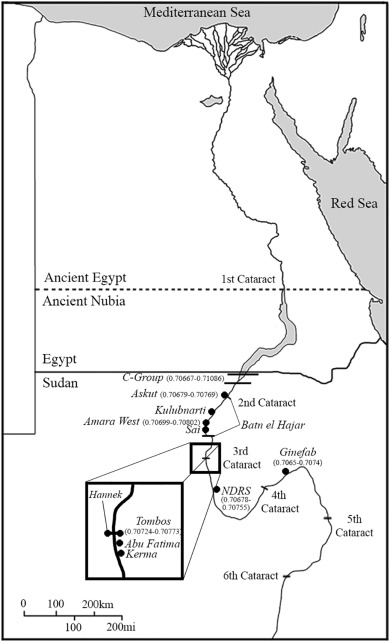
\includegraphics[width=0.45\textwidth]{egypt_regions.jpg}
    \caption{A map of Egypt, with the regions under study highlighted \citep{schrader2019} }
    \label{fig:egypt_regions}
\end{figure}

As much as archaeologists have studied ancient Egypt, we still know regrettably little.
One question that arises is how mobile ancient Egyptian society was.
So, \cite{schrader2019} investigated the movement of rural and urban settlements
in the Third Nile Cataract region of Egypt from 2500 BCE to 656 BCE.

To achieve this, the researchers took samples from graveyards in three settlements:
Tombos, Abu Fatima, and Hannek. The locations of these cities are shown on a map
in Figure~\ref{fig:egypt_regions}. These locations range from urban to rural and elite
to common. The
graveyard use at each location spanned nearly a thousand years. The researchers
then measured strontium isotope ratios of tooth enamel samples to
identify local and non-local skeletons.

The authors discovered that, across the board, numerous non-local skeletons were buried
alongside local ones. In the urban Abu Fatima and the rural Hannek, about 1/4 of
the skeletons sampled were non-local. In the urban Tombos, about 1/8 of sampled
skeletons were non-local. And, nearly all of the
non-local strontium ratios were consistent with strontium ratios found in the Second
Nile Cataract.

The researchers concluded that migration networks between the Second and Third
Nile Cataract not known before must have existed.
Further, it must have been normal
for migrants and locals to coexist since both groups were buried together in both
cemeteries for the elite such as Abu Fatima and cemeteries for commoners such
as Hannek. It is also notable that people across financial brackets migrated.
The researchers expressed that they could identify the exact origins of the non-local
individuals if their strontium results had more resolution, so they encouraged
future research to refine the Egyptian isoscape.

The work of \cite{schrader2019} illuminates the capability of strontium isotope analysis
to study the mobility of ancient peoples. The method can identify where migrants came
from and how frequently they migrated. However, strontium isotope analysis alone can
not reveal migration routes and levels of xenophobia, so it must be combined with tools such as
other archaeological data and historical accounts to get the best results. The research
article also points out the need for refining isoscapes. With more result resolution,
archaeologists can make more persuasive and impactful arguments with strontium isotope analysis data.


\section{Conclusion}
In conclusion, strontium isotope analysis emerges as a potent and illuminating
tool for delving into the mysteries of ancient Egypt. The method, which
discerns the geographic origins of humans and animals through the examination of
strontium isotope ratios in their remains, provides a unique lens into the past.

Through this paper, I've explored the foundations and applications of strontium
isotope analysis, particularly in the context of ancient Egypt. Strontium isotope
analysis reveals the historical mobility and migration patterns of ancient
populations, challenging conventional narratives and shedding light on the
dynamic nature of human societies. The ability to discern the provenance of
individuals, animals, and even crops enhances our understanding of trade,
societal structures, and environmental interactions.

Case studies, such as the investigation into the origins of the Hyksos and the
migrational patterns in ancient Egypt, exemplify the method's capacity to
rewrite historical interpretations. The study of mummified birds and the assessment of
migrational origins in
ancient Egypt showcase the breadth of insights that strontium isotope analysis
can provide.

Beyond the realm of archaeology, strontium isotope analysis extends its utility
to diverse fields. From forensics, where it aids in post-mortem investigations,
to conservation efforts by tracking the illegal trade of animal products, this
analytical method demonstrates its versatility and relevance.
Despite its strengths, strontium isotope analysis is not without
limitations. Challenges related to precision, accuracy, and cost underscore the
need for a nuanced approach and complementary methods.

Ongoing advancements in technology and techniques hold the
promise of overcoming these challenges, making strontium isotope analysis an
increasingly indispensable tool in the archaeologist's toolkit. As our
understanding of strontium isotope analysis continues to evolve, it opens
avenues for interdisciplinary research, encouraging collaboration between
archaeologists, chemists, and environmental scientists.

By deciphering the secrets embedded in skeletal remains and ancient artifacts,
strontium isotope analysis contributes significantly to reconstructing the
intricate tapestry of human history. Through this survey of strontium isotope
analysis in archaeological research of ancient Egypt, researchers uncover how
strontium isotope analysis can unravel the complexities of the past,
paving the way for a more nuanced and enriched narrative of human civilization.

\section{Acknowledgment}

This article was partially generated with assistance from ChatGPT, an OpenAI language model.


% Bibliography
\bibliographystyle{apalike}
\bibliography{references} % Specify your bibliography file (e.g., references.bib)

\end{document}
